\documentclass{book}

\input{../activities-preamble.tex}
\begin{document}
\setcounter{project}{36}
\addtocounter{project}{-1}
\begin{investigation}[]\label{investigation-6}
\hypertarget{p-351}{}%
Mapmakers in the fictional land of Euleria have drawn the borders of the various dukedoms of the land. To make the map pretty, they wish to color each region. Adjacent regions must be colored differently, but it is perfectly fine to color two distant regions with the same color. What is the fewest colors the mapmakers can use and still accomplish this task?%
\begin{sidebyside}{1}{0.25}{0.25}{0}
\begin{sbspanel}{0.5}
\resizebox{\linewidth}{!}{{
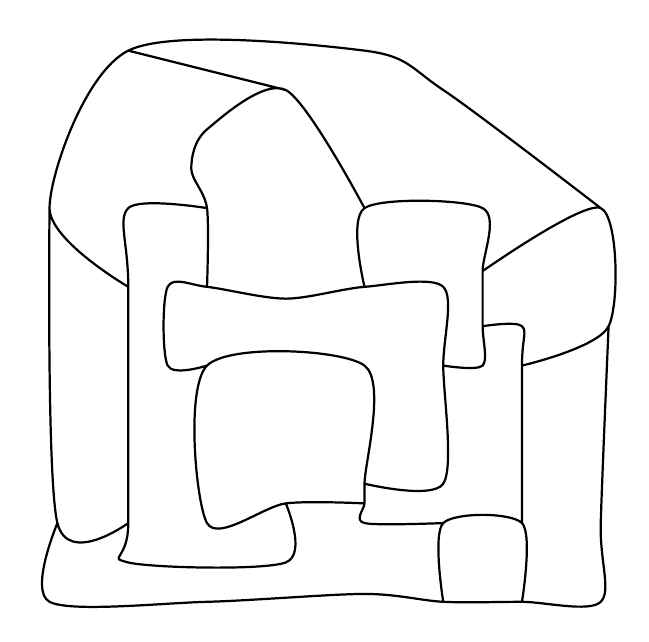
\begin{tikzpicture}
	\draw[thick]
		plot [smooth] coordinates {(0.1,1) (0,0) (2,0) (4,0.1) (5,0) (6,0) (7,0) (7,1) (7.1,3.5)}
		plot [smooth] coordinates {(1,1) (0.1,1) (0,5)}
		plot [smooth] coordinates {(2,5) (1,5) (1,4) (1,1) (1,.5) (3,.5) (3,1.25)}
		plot [smooth] coordinates {(5,0) (5,1) (6,1) (6,0)}
		plot [smooth] coordinates {(6,1) (6,3) (6,3.5) (5.5,3.5)}
		plot [smooth] coordinates {(5,1) (4,1) (4,1.25) (4,1.5) (4,3) (2,3) (2,1) (3,1.25) (4,1.25)}
		plot [smooth] coordinates {(4,1.5) (5,1.5) (5,3) (5,4) (4,4) (3,3.85) (2,4) (1.5,4) (1.5,3) (2,3)}
		plot [smooth] coordinates {(5,3) (5.5,3) (5.5,3.5) (5.5, 4.2) (5.5,5) (4,5) (4,4)}
		plot [smooth] coordinates {(6,3) (7.1, 3.5) (7,5) (5.5,4.2)}
		plot [smooth] coordinates {(7,5) (5,6.5) (4,7) (1,7) (0,5) (1,4)}
		plot [smooth] coordinates {(2,4) (2,5) (1.8,5.5) (2,6) (3,6.5) (4,5)}
		plot [smooth] coordinates {(1,7) (3,6.5)};
	\end{tikzpicture}
}
}
\end{sbspanel}
\end{sidebyside}
\end{investigation}
\end{document}
